\documentclass{article}
\usepackage{graphicx}                              %for PNG images (pdflatex)
\usepackage{graphics}                              %for EPS images (latex)
\usepackage[linkbordercolor={1.0 1.0 0.0}]{hyperref} %for \url tag
\usepackage{color}                                 %for defining custom colors
\usepackage{framed}                                %for shaded and framed paragraphs
\usepackage{textcomp}                              %for various symbols, e.g. Registered Mark
\usepackage{geometry}                              %for defining page size
\usepackage{longtable}                             %for breaking tables
%

%---CUSTOM FLOAT---
\usepackage{float}
\floatstyle{plain}
\newfloat{illustration}{htp}{loi}
\floatname{illustration}{Illustration}

%
\geometry{verbose,a4paper,tmargin=2.5cm,bmargin=2.5cm,lmargin=2.5cm,rmargin=2cm}
\hypersetup{
  pdfauthor = {Author Name},
  pdftitle = {Paper title},
  pdfsubject = {Paper subject},
  pdfkeywords = {Paper,keyword,comma-separated},
  pdfcreator = {PDFLaTeX with hyperref package},
  pdfproducer = {PDFLaTeX}
}
%
\bibliographystyle{IEEEtran}                       %a nice bibliography style
%
\def\efill{\hfill\nopagebreak}%
\hyphenation{Nordu-Grid}
\setlength{\parindent}{0cm}
\setlength{\FrameRule}{1pt}
\setlength{\FrameSep}{8pt}
\addtolength{\parskip}{5pt}
%\renewcommand{\thefootnote}{\fnsymbol{footnote}}
\renewcommand{\arraystretch}{1.3}
\newcommand{\dothis}{\colorbox{shadecolor}}
\newcommand{\globus}{Globus Toolkit\textsuperscript{\textregistered}~2~}
\newcommand{\GT}{Globus Toolkit\textsuperscript{\textregistered}}
\newcommand{\ngdl}{\url{http://download.nordugrid.org/}~}
\definecolor{shadecolor}{rgb}{1,1,0.6}
\definecolor{salmon}{rgb}{1,0.9,1}
\definecolor{bordeaux}{rgb}{0.75,0.,0.}
\definecolor{cyan}{rgb}{0,1,1}
%
%----- DON'T CHANGE HEADER MATTER
\begin{document}
\def\today{\number\day/\number\month/\number\year}

\begin{titlepage}

\begin{tabular}{rl}
\resizebox*{3cm}{!}{
\includegraphics{fig/logo-knowarc.png}}
\end{tabular}

\hrulefill

%-------- Change this to Knowarc_D<w>.<d>-<n>_<yy>

{\raggedleft Knowarc\_D0.0-0\_00\par}

{\raggedleft \today\par}

\vspace*{2cm}

%%%%---- The title ----
{\centering \textsc{\Large ARC1 Python Web Services Developer's Guide }\Large \par}
\vspace*{0.5cm}
    
%%%%---- A subtitle, if necessary ----
%{\centering \textit{\large Paper subtitle}\large \par}
    
\vspace*{1.5cm}
%%%%---- A list of authors ----
    {\centering \large Tam\'as Kazinczy\footnote{kazy@niif.hu} \large \par}
    
%%%%---- An abstract - if style is article ----
%\begin{abstract}
%The abstract
%\end{abstract}
\end{titlepage}

\tableofcontents
\newpage
\listoffigures
\newpage


\section{Preface}


\subsection{Purpose of this document}

This document has two main objectives. On one hand it guides you through the
creation of a new Python-based Web Service in ARC1\footnote[1]{See
  \url{http://svn.nordugrid.org/trac/nordugrid/browser/arc1/trunk/README}
  and \url{http://www.knowarc.eu/}}. On the other hand it describes the steps
needed to test the newly-created ARC1 Service.

The document has the following structure:

\begin{itemize}

  \item{In the first section we provide a brief description about the
    intended audience and the service to be implemented.}

  \item{In the next section Service Design will be discussed.}

  \item{In section Implementing the Service we provide an overview of the
    Python implementation.}

  \item{In section Putting GreetingService to work we describe the steps
    needed to make the Python service work.}

  \item{In section Testing the Service we introduce a tool to test the
    service with and the steps of testing.}

\end{itemize}

\subsection{Intended audience}

ARC1 Python Web Services Developer's Guide is intended for developers, who:

\begin{itemize}

  \item{have some experience with Python;}
  \item{want to create Python-based services in ARC1;}
  \item{are familiar with XML\footnote{See
      \url{http://www.w3.org/XML}}, XSD\footnote{See
      \url{http://www.w3.org/XML/Schema}}, SOAP\footnote{See
      \url{http://www.w3.org/TR/soap/}} and WSDL\footnote{See
      \url{http://www.w3.org/TR/wsdl} and
      \url{http://www.w3.org/TR/wsdl20}}.}

\end{itemize}

\subsection{About the service to be implemented}

The service (GreetingService) to be implemented is quite
simple. Users send their names to the service in a message and,
as an answer, they get a
personal greeting that tells them the local time on the server. So
if the name of the user is Anonymous, the answer would be something
like: 'Hello, Anonymous! Local time is: [Mon Aug 11 14:17:53 2008]'.

\newpage

\section{Service Design}

For the sake of clarity and the simplicity of testing, we use a
top-down approach in the service design. First, we create an XML
Schema Definition (XSD), then use this XSD to construct the WSDL of
the service.

\subsection{Designing the XML Schema Definition (XSD)}

The GreetingService is quite simple: it has a single input and a single output.
As an input, it takes a full personal name; as an output, it sends a
greeting message in the following form: “Hello, XY! Local time is:
[SERVER-DATE-AND-TIME]”.

In designing the service first, we provide a targetNamespace for the schema. 
Let it be, for example \linebreak
\verb#http://example.com/GreetingService/types#. We also define a 
namespace prefix \verb#tns# for this namespace so that we can refer to 
the types defined in this schema.

\begin{illustration}
\begin{center}
\begin{tabular}{|l|}
\hline
\verb#<schema#\\
\verb#  targetNamespace="http://example.com/GreetingService/types"#\\
\verb#  xmlns="http://www.w3.org/2001/XMLSchema"#\\
\verb#  xmlns:xsd="http://www.w3.org/2001/XMLSchema"#\\
\verb#  xmlns:tns="http://example.com/GreetingService/types"#\\
\verb#  elementFormDefault="qualified">#\\
\hline
\end{tabular}
\end{center}
\caption{Definition of target namespace}
\end{illustration}

Next, we create simple types for the input (name) and output (greeting).

\begin{illustration}
\begin{center}
\begin{tabular}{|l|}
\hline
\verb#<simpleType name="name">#\\
\verb#  <restriction base="xsd:string"/>#\\
\verb#</simpleType>#\\

\verb#<simpleType name="greeting">#\\
\verb#  <restriction base="xsd:string"/>#\\
\verb#</simpleType>#\\
\hline
\end{tabular}
\end{center}
\caption{Simple types for input (name) and output (greeting)}
\end{illustration}

GreetingService is of a request-response type, so we create types for
the request and response as well.

\begin{illustration}
\begin{center}
\begin{tabular}{|l|}
\hline
\verb#<complexType name="GreetingServiceRequestType">#\\ 
\verb#  <sequence>#\\ 
\verb#    <element name="yourName" type="tns:name" minOccurs="1" maxOccurs="1"/>#\\ 
\verb#  </sequence>#\\ 
\verb#</complexType>#\\
\hline
\end{tabular}
\end{center}
\caption{Complex type to represent request}
\end{illustration}

\begin{illustration}
\begin{center}
\begin{tabular}{|l|}
\hline
\verb#<complexType name="GreetingServiceResponseType">#\\ 
\verb#  <sequence>#\\ 
\verb#    <element name="yourGreeting" type="tns:greeting" minOccurs="1" maxOccurs="1"/>#\\ 
\verb#  </sequence>#\\ 
\verb#</complexType>#\\
\hline
\end{tabular}
\end{center}
\caption{Complex type to represent response}
\end{illustration}

\pagebreak

Here we have used the previously created simple types (referred to as
\verb#tns:name# and \verb#tns:greeting#) to define the elements
\verb#yourName# and \verb#yourGreeting# of complex types that will
represent the request and response.

All we need to do now is to create the request and response elements
which are of complex types mentioned before.

\begin{illustration}
\begin{center}
\begin{tabular}{|l|}
\hline
\verb#<element name="GreetingServiceRequest" type="tns:GreetingServiceRequestType"/>#\\ 
\verb#<element name="GreetingServiceResponse" type="tns:GreetingServiceResponseType"/>#\\ 
\hline
\end{tabular}
\end{center}
\caption{Request and response element}
\end{illustration}

The complete XSD can be found in Appendix \ref{app:xsd} of this guide.

%\clearpage

\subsection{Designing the Service WSDL}

Construction of the service WSDL is relatively straightforward.

We use those elements defined in our XML schema so we have to
provide a namespace prefix for the namespace
\verb#http://example.com/GreetingService/types# to be able to refer to
them. We also define the target namespace
(\verb#http://example.com/GreetingService#) as well as a prefix for
our service definition.

\begin{illustration}
\begin{center}
\begin{tabular}{|l|}
\hline
\verb#<definitions#\\ 
\verb#  targetNamespace="http://example.com/GreetingService"#\\ 
\verb#  xmlns="http://schemas.xmlsoap.org/wsdl/"#\\ 
\verb#  xmlns:xsd="http://www.w3.org/2001/XMLSchema"#\\ 
\verb#  xmlns:soap="http://schemas.xmlsoap.org/wsdl/soap/"#\\ 
\verb#  xmlns:wsdl="http://schemas.xmlsoap.org/wsdl/"#\\ 
\verb#  xmlns:gs="http://example.com/GreetingService"#\\ 
\verb#  xmlns:gst="http://example.com/GreetingService/types">#\\
\hline
\end{tabular}
\end{center}
\caption{Namespaces}
\end{illustration}

\pagebreak

We also need to import our XML schema in the
types section. It is worth noting that (according to the WS-I
Basic Profile Version 1.1): ``To import XML Schema Definitions, a
DESCRIPTION MUST use the XML Schema \texttt{import} statement.''

\begin{illustration}
\begin{center}
\begin{tabular}{|l|}
\hline
\verb#<wsdl:types>#\\ 
\verb#  <xsd:schema xmlns:xsd="http://www.w3.org/2001/XMLSchema">#\\
\verb#    <xsd:import namespace="http://example.com/GreetingService/types"#\\
\verb#                schemaLocation="GreetingService.xsd"/>#\\ 
\verb#  </xsd:schema>#\\ 
\verb#</wsdl:types>#\\
\hline
\end{tabular}
\end{center}
\caption{Types}
\end{illustration}

Then, we create the messages to be used by the service. These messages
will use the request and response elements that we created earlier in the
schema.

\begin{illustration}
\begin{center}
\begin{tabular}{|l|}
\hline
\verb#<wsdl:message name="GreetingServiceRequestMessage">#\\ 
\verb#  <wsdl:part name="payload" element="gst:GreetingServiceRequest"/>#\\ 
\verb#</wsdl:message>#\\ 

\verb#<wsdl:message name="GreetingServiceResponseMessage">#\\ 
\verb#  <wsdl:part name="payload" element="gst:GreetingServiceResponse"/>#\\ 
\verb#</wsdl:message>#\\
\hline
\end{tabular}
\end{center}
\caption{Definition of WSDL messages}
\end{illustration}

The next step is to create a portType. Here we define the operation (greet)
along with its input and output messages.

\begin{illustration}
\begin{center}
\begin{tabular}{|l|}
\hline
\verb#<wsdl:portType name="GreetingServicePT">#\\ 
\verb#  <wsdl:operation name="greet">#\\ 
\verb#    <wsdl:input name="GreetingServiceInput"#\\ 
\verb#                message="gs:GreetingServiceRequestMessage"/>#\\ 
\verb#    <wsdl:output name="GreetingServiceOutput"#\\ 
\verb#                 message="gs:GreetingServiceResponseMessage"/>#\\ 
\verb#  </wsdl:operation>#\\ 
\verb#</wsdl:portType>#\\ 
\hline
\end{tabular}
\end{center}
\caption{Definition of WSDL portType}
\end{illustration}

\pagebreak

Then we define the binding where we use the portType created previously. 
The key point here is that we use \texttt{document/literal}
style SOAP HTTP binding.

\begin{illustration}
\begin{center}
\begin{tabular}{|l|}
\hline
\verb#<wsdl:binding name="GreetingServiceBinding" type="gs:GreetingServicePT">#\\ 
\verb#  <soap:binding style="document" transport="http://schemas.xmlsoap.org/soap/http"/>#\\ 
\verb#  <wsdl:operation name="greet">#\\ 
\verb#    <soap:operation soapAction="greet"/>#\\ 
\verb#    <wsdl:input name="GreetingServiceInput">#\\ 
\verb#      <soap:body use="literal"/>#\\ 
\verb#    </wsdl:input>#\\ 
\verb#    <wsdl:output name="GreetingServiceOutput">#\\ 
\verb#      <soap:body use="literal"/>#\\
\verb#    </wsdl:output>#\\ 
\verb#  </wsdl:operation>#\\ 
\verb#</wsdl:binding>#\\
\hline
\end{tabular}
\end{center}
\caption{Definition of WSDL binding}
\end{illustration}

As the last step of the design, we define the service with a port that 
uses this binding. For the sake of simplicity, we should provide an 
endpoint address where our service will listen.

\begin{illustration}
\begin{center}
\begin{tabular}{|l|}
\hline
\verb#<wsdl:service name="GreetingService">#\\
\verb#  <wsdl:port name="GreetingServicePort" binding="gs:GreetingServiceBinding">#\\
\verb#    <soap:address location="http://arctest.ki.iif.hu:50000/GreetingService"/>#\\
\verb#  </wsdl:port>#\\
\verb#</wsdl:service>#\\
\hline
\end{tabular}
\end{center}
\caption{Definition of WSDL service}
\end{illustration}

The complete WSDL can be found in Appendix \ref{app:wsdl} of this guide.

\clearpage
\newpage

\section{Implementing the Service}

\subsection{Before jumping in}

Though configuration is discussed later in this document, some points
need prior explanation.

For demonstration purposes, fixed parts of the greeting of
GreetingService are stored in ARC HED's\footnote[1]{HED: Hosting
  Environment Daemon} XML configuration file. In the implementation we
will get these parts from the XML right after the instantiation of the
Python class (in the \verb#__init__()# method).

\subsection{Overview of the Python implementation}

As it was pointed out before, we get fixed parts of the greeting in the
\verb#__init__()# method. This also includes resolving the namespace
prefix of the service namespace \verb#http://example.com/GreetingService#.

In ARC1, Python-based services use a wrapper to access the core service
classes and their methods.
This means that upon starting ARC HED, the wrapper loads the Python based
services as modules. The nature of this wrapper indicates that every
such (Python based) service is required to provide a process()
method. In this method, we get the payload from the incoming SOAP
message, get the name of the consumer, get the local time, then construct
the greeting message, assemble the outgoing SOAP message and finally
return.

The source code including comments can be found in Appendix \ref{app:pysrc}
of this guide.

\newpage

\section{Putting GreetingService to work}

\subsection{Creating \texttt{\_\_init\_\_.py}}

Let us assume that our Python implementation (greetingservice.py)
resides in a directory called GreetingService\footnote[1]{
This directory is required to be under ARC1 home directory ($\$ARC1\_HOME$)}. 
Without \verb#__init__.py# in it, this is only a simple directory; it is
\verb#__init__.py# what makes GreetingService a Python package, so we
need to have one, even if it is an empty file.

\subsection{Creating \texttt{Makefile.am}}

We need \verb#Makefile.am# to generate the \verb#Makefile#. It is
rather simple in our example, consisting of only three lines:

\begin{illustration}
\begin{center}
\begin{tabular}{|l|}
\hline
\verb#pythondir= $(PYTHON_SITE_PACKAGES)/GreetingService#\\ 

\verb#python_DATA = __init__.py greetingservice.py#\\ 

\verb#EXTRA_DISTS = $(python_DATA)#\\
\hline
\end{tabular}
\end{center}
\caption{Contents of \texttt{Makefile.am}}
\end{illustration}

The first line tells where GreetingService will be installed. Here
\verb#$(PYTHON_SITE_PACKAGES)# refers to something like
\verb#/usr/local/lib/python2.5/site-packages/#.

Second line tells what the Python sources are (here you see the Python
source files separated by spaces) and the third one that we will use
these files in our service.

\subsection{Generating the \texttt{Makefile}}

Open a terminal, go to ARC1 home directory (\verb#$ARC1_HOME#), then
edit \verb#./configure.ac# (you may need root privileges to do this):

\begin{enumerate}

\item search for the text \verb#AC_CONFIG_FILES#;

\item put an extra path there for the \verb#GreetingService#
  \verb#Makefile# (this is required to be the relative path from
  \verb#$ARC1_HOME#, so if the \verb#GreetingService# directory was in
  \verb#$ARC1_HOME/src/services# then it should be
  \verb#src/services/GreetingService/Makefile#).

\end{enumerate}

After saving configure.ac run `\verb#./autogen.sh#` and
`\verb#./configure#` in this order as in case of ordinary ARC1 configuration (doing this needs root privileges).

\clearpage

\subsection{Configuring the ARC HED}

Edit ARC1's XML configuration file used when starting ARC HED.

We define the \verb#http://example.com/GreetingService# namespace in
the \verb#<ArcConfig># node (see below), as we also use this
configuration file to store fixed parts of the greeting of
\verb#GreetingService#.

\begin{illustration}
\begin{center}
\begin{tabular}{|l|}
\hline
\verb#<ArcConfig#\\ 
\verb#  xmlns="http://www.nordugrid.org/schemas/ArcConfig/2007"#\\
\verb#  xmlns:tcp="http://www.nordugrid.org/schemas/ArcMCCTCP/2007"#\\
\verb#  xmlns:arex="http://www.nordugrid.org/schemas/a-rex/Config"#\\
\verb#  xmlns:gsrv="http://example.com/GreetingService">#\\
\hline
\end{tabular}
\end{center}
\caption{Definition of service namespace in ArcConfig node}
\end{illustration}

We have to create a new \verb#<Service># node in \verb#<Chain># to
represent our service.

\begin{illustration}
\begin{center}
\begin{tabular}{|l|}
\hline
\verb#<Service name="pythonservice" id="greetingservice">#\\ 
\verb#  <ClassName>GreetingService.greetingservice.GreetingClass</ClassName>#\\ 
\verb#  <gsrv:part1>Hello, </gsrv:part1>#\\ 
\verb#  <gsrv:part2>! Local time is: [</gsrv:part2>#\\ 
\verb#  <gsrv:part3>]</gsrv:part3>#\\ 
\verb#</Service>#\\
\hline
\end{tabular}
\end{center}
\caption{Definition of service in ARC HED}
\end{illustration}

As mentioned before, Python-based services are handled through a
wrapper. This wrapper is called \linebreak{}\verb#pythonservice#, that is where the
name attribute of \verb#<Service># node comes from.

ClassName consists of three parts, separated by periods. The first
part refers to the package \linebreak{}(\verb#GreetingService# here), the second
part refers to the Python module (\verb#greetingservice# here -- so
the Python source file is \verb#greetingservice.py#) while the third
one is the name of the Python Class \linebreak{}(\verb#GreetingClass#).

The next three nodes (\verb#<gsrv:part1>#, \verb#<gsrv:part2># and
\verb#<gsrv:part3>#) are the fixed parts of the greeting.

All we have to do now is to check the \verb#<Component># nodes (so we
have TCP, HTTP, SOAP and POST present in the HTTP component), then
create a new node for \verb#GreetingService# in \verb#<Plexer>#.

\begin{illustration}
\begin{center}
\begin{tabular}{|l|}
\hline
\verb#<Plexer name="plexer.service" id="plexer">#\\
\verb#  <next id="a-rex">^/arex$</next>#\\
\verb#  <next id="count">^/count$</next>#\\
\verb#  <next id="greetingservice">^/GreetingService$</next>#\\
\verb#</Plexer>#\\
\hline
\end{tabular}
\end{center}
\caption{Configuration of Plexer}
\end{illustration}

The new node tells that the Service, whose ID is
\verb#greetingservice#, will be made accessible at the relative URL
\verb#/GreetingService#.

\subsection{Installation}

Installation of the service is also straightforward. Open a terminal, go to
the directory of the service (for example
\verb#$ARC1_HOME/src/services/GreetingService#) and execute the
command: `\verb#make install#` (doing this may need root privileges).
After the execution of the command ARC HED needs to be restarted.

\newpage

\section{Testing the Service}

The top-down design approach helps us to test
\verb#GreetingService#. There are several Open Source tools that can help
to test the service without having to write a client for it.

Basically, when considering which tool to use, we look for the
following features:

\begin{itemize}
  \item{capability of sending SOAP messages and receiving answers;}
  \item{capability of checking XML schema compliance;}
  \item{capability of generating message from WSDL;}
  \item{possibility of using custom assertions;}
  \item{possibility of using parameters.}
\end{itemize}

Our choice for testing the service had been soapUI. It is a widely used open
source tool for Web Service Testing that has all the features (even
more) we need.

\subsection{Creating the Test Project}
\label{sec:createtp}

After starting soapUI, we can create a new WSDL project by pressing
Ctrl+N or selecting \textit{New WSDL Project} from the \textit{File}
menu. [See \emph{Figure \ref{fig:newwsdl}}]

\begin{figure}[!hbp]
\begin{center}
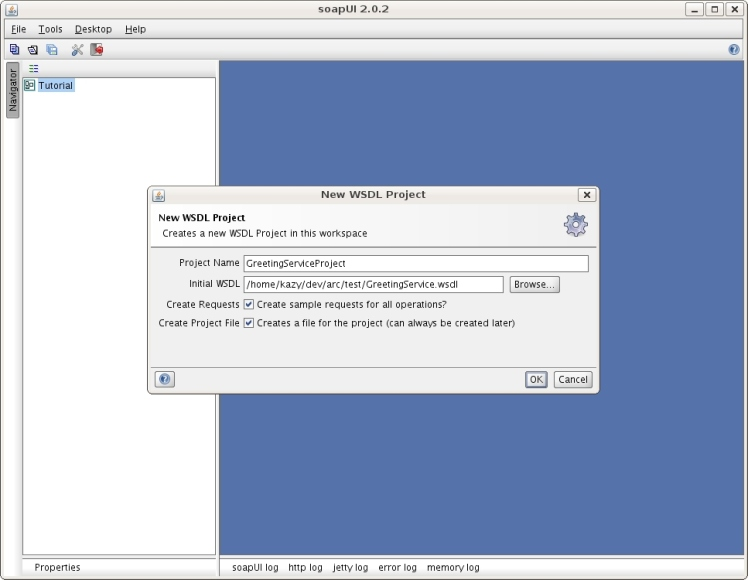
\includegraphics{fig/ARC1PythonDGDraft-img2_resize.jpg}
\caption{New WSDL Project}
\label{fig:newwsdl}
\end{center}
\end{figure}

Fill in the \textit{Project Name} (it could be any of your choice) and
browse for the WSDL that we created before. You should leave
\textit{Create Requests} checked. This means that requests are
automatically generated from the WSDL. You may also check the
\textit{Create Project File} checkbox as it will allow you to save
your project.

\subsection{Adding the Test Request to a Test Case}
\label{sec:addtr2tc}

Now you should see the project in the \textit{Navigator
  view}. Navigate to \textit{Request 1} in the tree and open it (press
Enter or select \textit{Show Request Editor} from the context
menu). [See \emph{Figure \ref{fig:showreqed}}]

\begin{figure}[!hbp]
\begin{center}
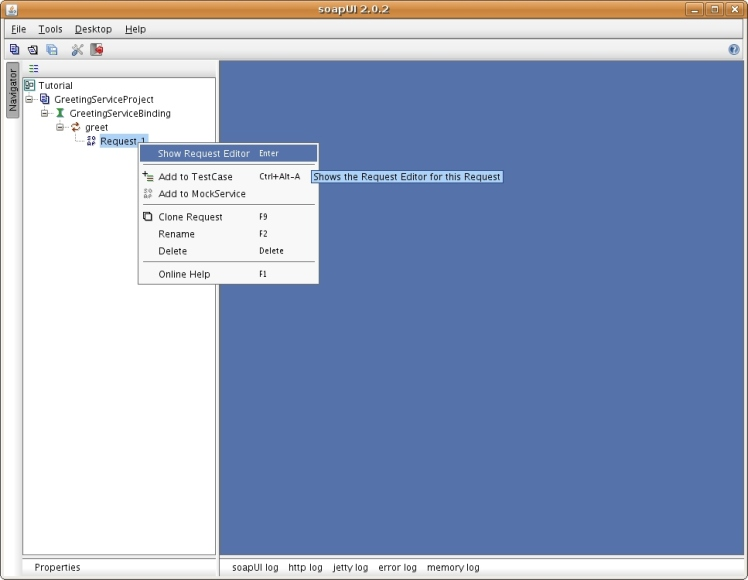
\includegraphics{fig/ARC1PythonDGDraft-img3_resize.jpg}
\caption{Show Request Editor}
\label{fig:showreqed}
\end{center}
\end{figure}

Next we add this request to a Test Case. Click on the second icon from
the left in the Request Editor (tooltip says: Adds this request to a
TestCase). [See \emph{Figure \ref{fig:addreq2tc}}]

\begin{figure}
\begin{center}
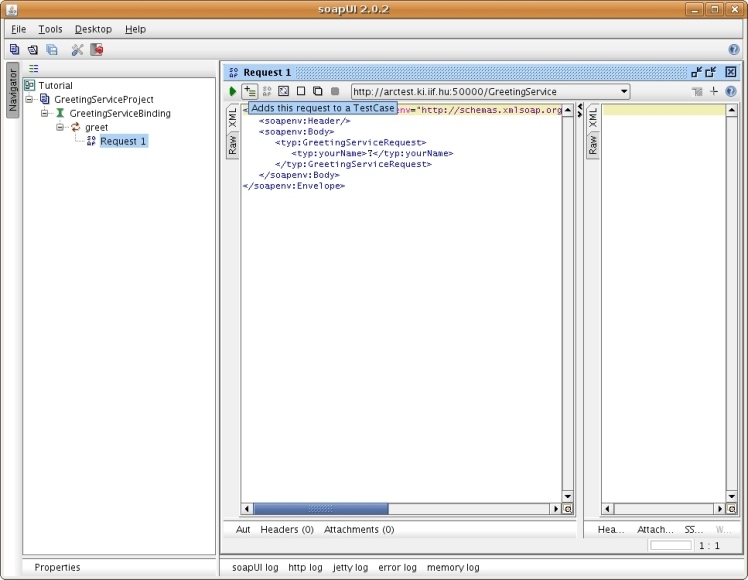
\includegraphics{fig/ARC1PythonDGDraft-img4_resize.jpg}
\caption{Adding Request to a Test Case 1}
\label{fig:addreq2tc}
\end{center}
\end{figure}

As we do not have a Test Suite yet, we need to create a Test Suite as
well. Choose a name for your Test Suite and Test Case (e.g.:
GreetingServiceTS and GreetingServiceTC1).

Now, a window appears. Here you can specify the name of the request
(e.g.: greetRequest1) and add predefined assertions. For example, you
may opt in the \textit{Add Schema Assertion} checkbox to validate
messages against our XML schema. [See \emph{Figure \ref{fig:addreq2tc2}}]

\begin{figure}
\begin{center}
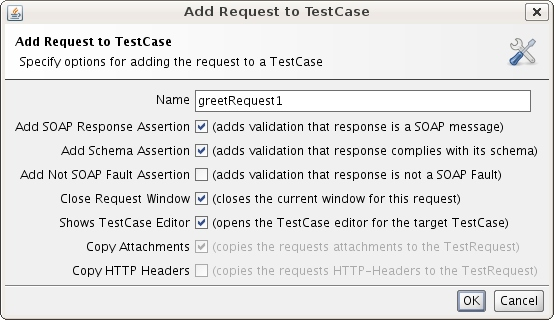
\includegraphics{fig/ARC1PythonDGDraft-img5.jpg}
\caption{Adding Request to a Test Case 2}
\label{fig:addreq2tc2}
\end{center}
\end{figure}

You should leave \textit{Show TestCase Editor} checked as we will
edit the Test Case in the following step.

\subsection{Editing the Test Case}
\label{sec:edittc}

After the Test Case Editor appears, click on greetRequest and select
\textit{Insert Step} $\to$ \textit{Properties} in the context menu
(tooltip says: Defines / Loads global TestCase properties). [See 
\emph{Figure \ref{fig:insprop}}]

\begin{figure}[!hbp]
\begin{center}
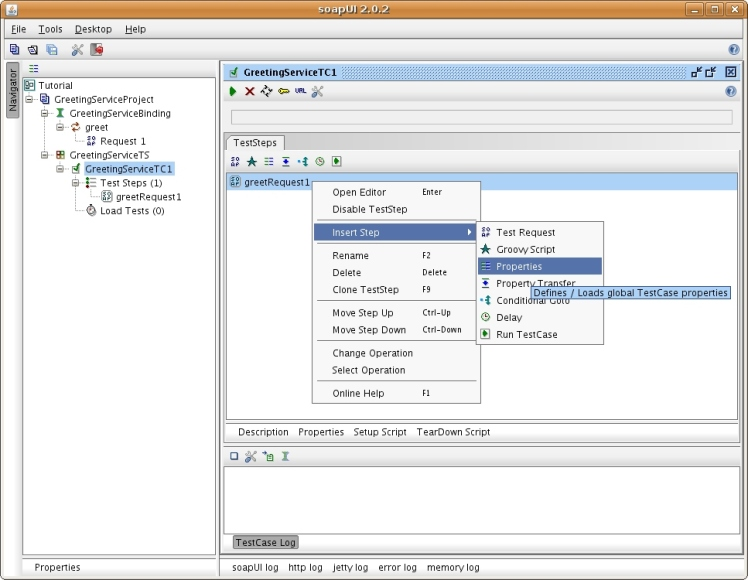
\includegraphics{fig/ARC1PythonDGDraft-img6_resize.jpg}
\caption{Insert Properties}
\label{fig:insprop}
\end{center}
\end{figure}

Fill in the name of the step (e.g.: greetProperties). The properties
window shows up. It has a table with two columns (Name and
Value). Here you can add a property (e.g.: inputName) by clicking on
the first icon from the left (tooltip says: Adds a property to the
property list) that could be used in the request and in assertions as
well. [See \emph{Figure \ref{fig:addprop1}} and \emph{Figure \ref{fig:addprop2}}]

\begin{figure}[!hbp]
\begin{center}
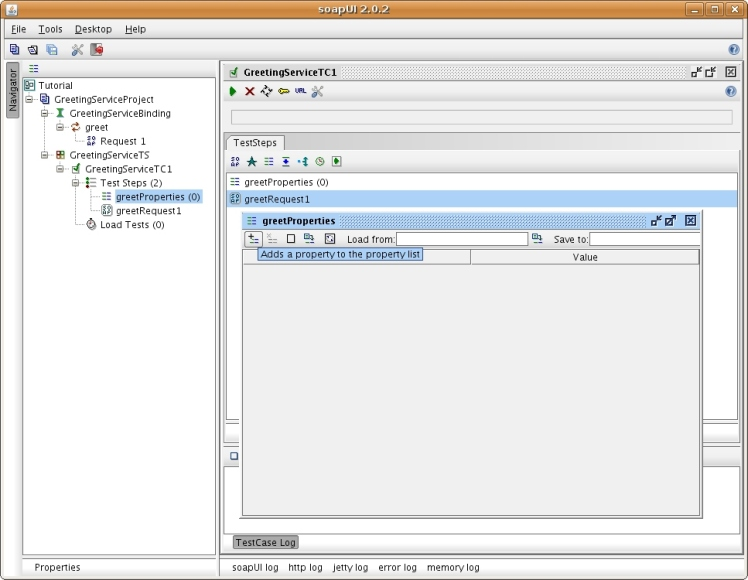
\includegraphics{fig/ARC1PythonDGDraft-img7_resize.jpg}
\caption{Adding a Property 1}
\label{fig:addprop1}
\end{center}
\end{figure}

\begin{figure}[!hbp]
\begin{center}
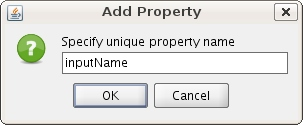
\includegraphics{fig/ARC1PythonDGDraft-img8.jpg}
\caption{Adding a Property 2}
\label{fig:addprop2}
\end{center}
\end{figure}

Close the properties window after adding the property (and providing a
value for it). [See \emph{Figure \ref{fig:addprop3}}]

\begin{figure}
\begin{center}
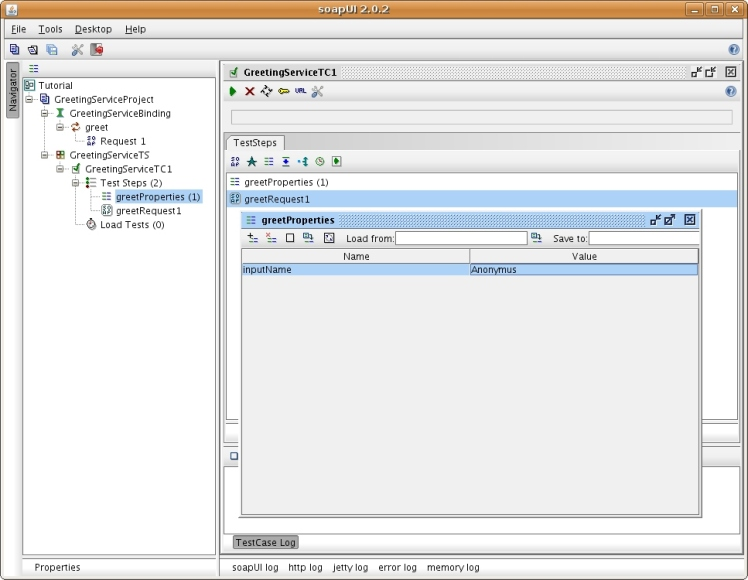
\includegraphics{fig/ARC1PythonDGDraft-img9_resize.jpg}
\caption{Adding a Property 3}
\label{fig:addprop3}
\end{center}
\end{figure}

Now double click on greetRequest1; this opens the Request Editor. In
\verb#<yourName>#, write \verb#${inputName}# instead of the default value
(a question mark).

\subsection{Assertions}
\label{sec:assertions}

Still in the Request Editor, click on the second icon from the left
(tooltip says: Adds an assertion to this item). [See \emph{Figure \ref{fig:assert1}}]

\begin{figure}[!hbp]
\begin{center}
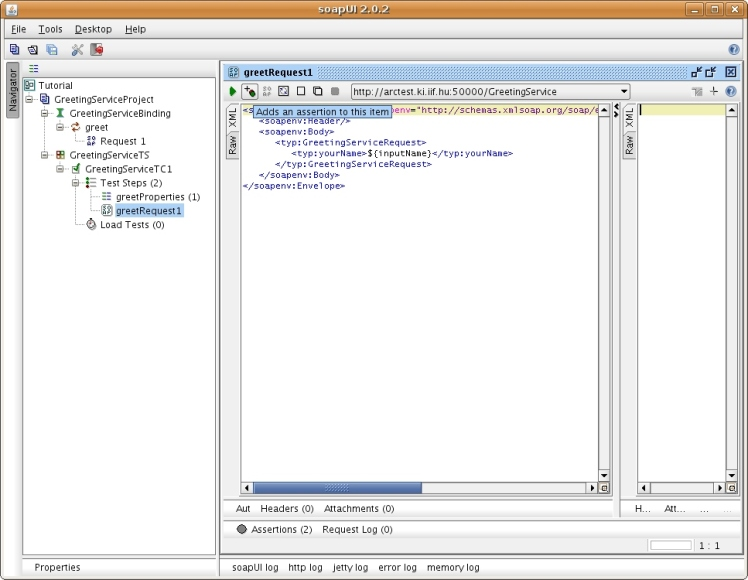
\includegraphics{fig/ARC1PythonDGDraft-img10_resize.jpg}
\caption{Adding an Assertion 1}
\label{fig:assert1}
\end{center}
\end{figure}

Next, you have to choose the type of assertion. For now, this should
be \textit{Contains}. [See \emph{Figure \ref{fig:assert2}}]

\begin{figure}[!hbp]
\begin{center}
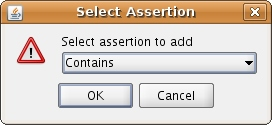
\includegraphics{fig/ARC1PythonDGDraft-img11.jpg}
\caption{Adding an Assertion 2}
\label{fig:assert2}
\end{center}
\end{figure}

In the next step, \textit{Content} should be
``\verb#Hello, ${inputName}!#'', so if we were to provide
``Anonymous'' as the value of \verb#inputName#, we could require the
answer to contain ``Hello, Anonymous!''. [See \emph{Figure \ref{fig:assert3}}]

\begin{figure}[!hbp]
\begin{center}
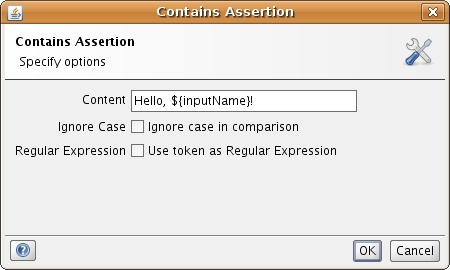
\includegraphics{fig/ARC1PythonDGDraft-img12.jpg}
\caption{Adding an Assertion 3}
\label{fig:assert3}
\end{center}
\end{figure}

\subsection{Running the Test Case}
\label{sec:runtc}

Close the Request Editor. In the Test Case Editor, click on the first
icon from the left (tooltip says: Runs this testcase). [See 
\emph{Figure \ref{fig:runtc}}]

\begin{figure}[!hbp]
\begin{center}
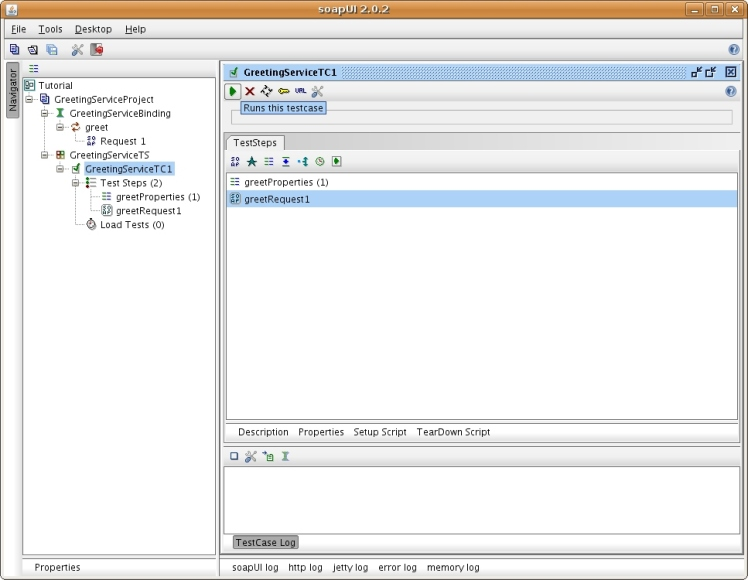
\includegraphics{fig/ARC1PythonDGDraft-img13_resize.jpg}
\caption{Running the Test Case}
\label{fig:runtc}
\end{center}
\end{figure}

\subsection{Evaluating Results}
\label{sec:evalresults}

If nothing went wrong, you would see the text FINISHED on a green
stripe. Details of the results are shown in the \textit{TestCase Log}.
[See \emph{Figure \ref{fig:tcresult}}]

\begin{figure}[!hbp]
\begin{center}
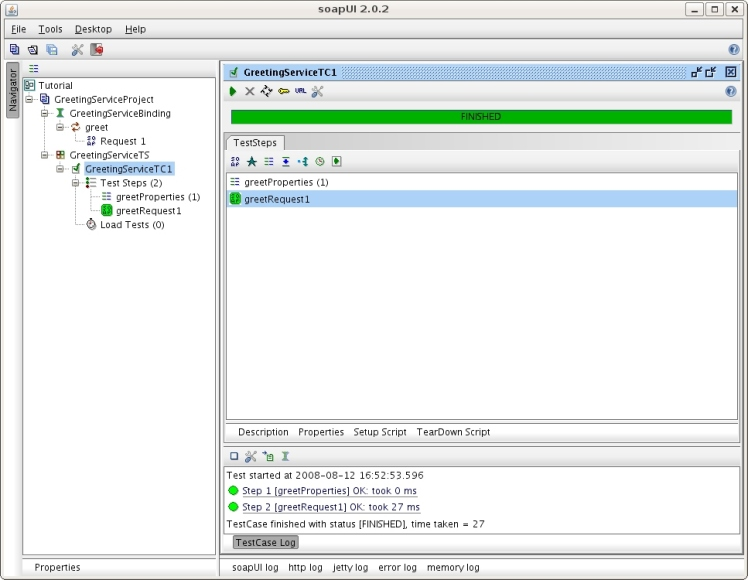
\includegraphics{fig/ARC1PythonDGDraft-img14_resize.jpg}
\caption{Test Case Results}
\label{fig:tcresult}
\end{center}
\end{figure}

Double clicking greetRequest1 allows you see the request and response
message and the results of assertions as well. [See \emph{Figure \ref{fig:respmsg}} 
and \emph{Figure \ref{fig:evalres}}]

\begin{figure}[!hbp]
\begin{center}
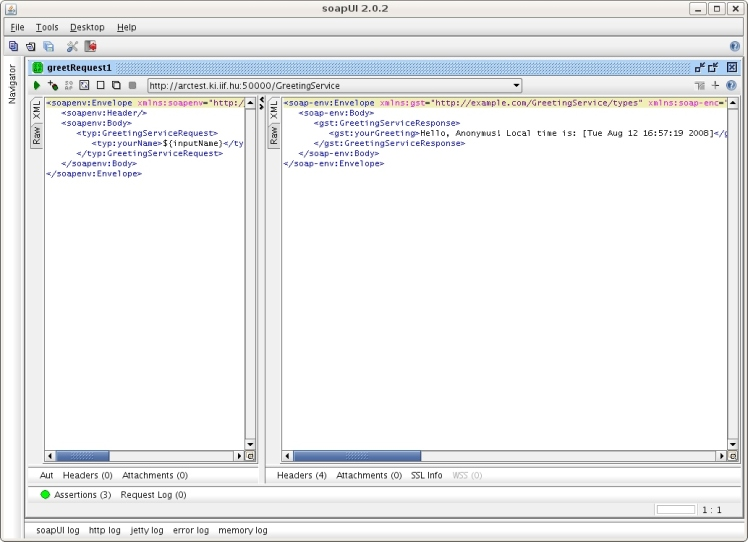
\includegraphics{fig/ARC1PythonDGDraft-img15_resize.jpg}
\caption{Response Message}
\label{fig:respmsg}
\end{center}
\end{figure}

\begin{figure}[!hbp]
\begin{center}
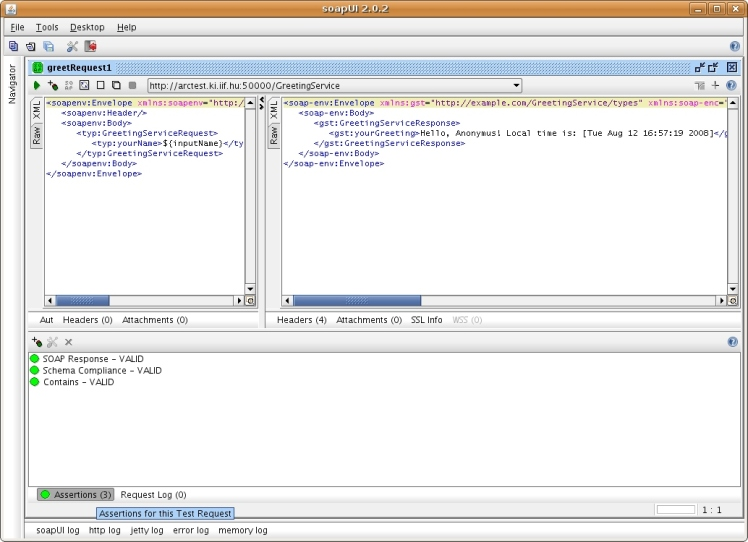
\includegraphics{fig/ARC1PythonDGDraft-img16_resize.jpg}
\caption{Assertions}
\label{fig:evalres}
\end{center}
\end{figure}

Although the value of the inputName property is not shown in the request
message, if you open the \textit{http log}, you will see that the
correct value has been used while creating the outgoing
request. [See \emph{Figure \ref{fig:httplog}}]

\begin{figure}
\begin{center}
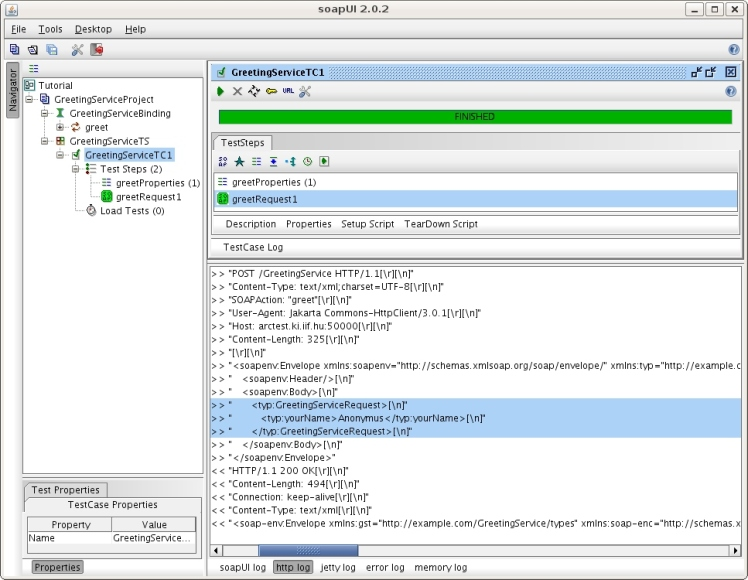
\includegraphics{fig/ARC1PythonDGDraft-img17_resize.jpg}
\caption{HTTP Log}
\label{fig:httplog}
\end{center}
\end{figure}

\clearpage
\newpage

\appendix

\section{Appendices}

\subsection{GreetingService.xsd}
\label{app:xsd}

\begin{verbatim}
<?xml version="1.0" encoding="UTF-8"?> 
<schema 
  targetNamespace="http://example.com/GreetingService/types"
  xmlns="http://www.w3.org/2001/XMLSchema"
  xmlns:xsd="http://www.w3.org/2001/XMLSchema"
  xmlns:tns="http://example.com/GreetingService/types"
  elementFormDefault="qualified">
	
  <simpleType name="name">
    <restriction base="xsd:string"/>
  </simpleType>

  <simpleType name="greeting">
    <restriction base="xsd:string"/>
  </simpleType>

  <complexType name="GreetingServiceRequestType">
    <sequence>
        <element name="yourName" type="tns:name" 
                 minOccurs="1" maxOccurs="1"/>
    </sequence>
  </complexType>

  <complexType name="GreetingServiceResponseType">
    <sequence>
      <element name="yourGreeting" type="tns:greeting" 
               minOccurs="1" maxOccurs="1"/>
    </sequence>
  </complexType>

  <element name="GreetingServiceRequest" 
           type="tns:GreetingServiceRequestType"/>
  <element name="GreetingServiceResponse" 
           type="tns:GreetingServiceResponseType"/>
</schema>
\end{verbatim}

\subsection{GreetingService.wsdl}
\label{app:wsdl}

\begin{verbatim}
<?xml version="1.0"
 encoding="UTF-8"?>
<definitions
  targetNamespace="http://example.com/GreetingService"
  xmlns="http://schemas.xmlsoap.org/wsdl/"
  xmlns:xsd="http://www.w3.org/2001/XMLSchema"
  xmlns:soap="http://schemas.xmlsoap.org/wsdl/soap/"
  xmlns:wsdl="http://schemas.xmlsoap.org/wsdl/"
  xmlns:gs="http://example.com/GreetingService"
  xmlns:gst="http://example.com/GreetingService/types">

  <wsdl:types> 
    <xsd:schema xmlns:xsd="http://www.w3.org/2001/XMLSchema"> 
      <xsd:import namespace="http://example.com/GreetingService/types" 
                  schemaLocation="GreetingService.xsd"/> 
    </xsd:schema> 
  </wsdl:types> 

  <wsdl:message name="GreetingServiceRequestMessage"> 
    <wsdl:part name="payload" element="gst:GreetingServiceRequest"/> 
  </wsdl:message> 

  <wsdl:message name="GreetingServiceResponseMessage"> 
    <wsdl:part name="payload" element="gst:GreetingServiceResponse"/> 
  </wsdl:message>

  <wsdl:portType name="GreetingServicePT"> 
    <wsdl:operation name="greet"> 
      <wsdl:input name="GreetingServiceInput"
                  message="gs:GreetingServiceRequestMessage"/> 
      <wsdl:output name="GreetingServiceOutput" 
                   message="gs:GreetingServiceResponseMessage"/> 
    </wsdl:operation> 
  </wsdl:portType> 

  <wsdl:binding name="GreetingServiceBinding" type="gs:GreetingServicePT"> 
    <soap:binding style="document" 
                  transport="http://schemas.xmlsoap.org/soap/http"/> 
    <wsdl:operation name="greet"> 
      <soap:operation soapAction="greet"/> 
      <wsdl:input name="GreetingServiceInput"> 
        <soap:body use="literal"/> 
      </wsdl:input> 
      <wsdl:output name="GreetingServiceOutput"> 
        <soap:body use="literal"/> 
      </wsdl:output> 
    </wsdl:operation> 
  </wsdl:binding> 

  <wsdl:service name="GreetingService"> 
    <wsdl:port name="GreetingServicePort" 
               binding="gs:GreetingServiceBinding"> 
      <soap:address location="http://arctest.ki.iif.hu:50000/GreetingService"/> 
    </wsdl:port> 
  </wsdl:service> 

</definitions>
\end{verbatim}

\subsection{greetingservice.py}
\label{app:pysrc}

\begin{verbatim}
import arc
import time

class GreetingClass:

    def __init__(self, cfg):
        # we want to use members of the 'http://example.com/GreetingService' namespace
        # so we need to know which namespace prefix was assigned to it
        # we get the namespace prefix into 'self.gs_ns'
        self.gs_ns = cfg.NamespacePrefix('http://example.com/GreetingService')

        # get part1 of greeting from the config XML
        self.part1 = str(cfg.Get(self.gs_ns + ':part1'))

        # get part2 of greeting from the config XML
        self.part2 = str(cfg.Get(self.gs_ns + ':part2'))

        # get part3 of greeting from the config XML
        self.part3 = str(cfg.Get(self.gs_ns + ':part3'))

    def process(self, inmsg, outmsg):

        # get the payload from the message
        inpayload = inmsg.Payload()

        # we want to use members of the 'http://example.com/GreetingService/types'
        # namespace so we need to know which namespace prefix was assigned to it
        # we get the namespace prefix into a variable named 'gst_ns'
        gst_ns = inpayload.NamespacePrefix('http://example.com/GreetingService/types')

        # then we can get 'gst_ns:GreetingServiceRequest/gst_ns:yourName'
        GreetingServiceRequest = inpayload.Get(gst_ns + ':GreetingServiceRequest')

        name = str(GreetingServiceRequest.Get(gst_ns + ':yourName'))

        localtime = time.localtime()

        strlocaltime = time.asctime(localtime)

        # forge the greeting message
        greet = self.part1 + name + self.part2 + strlocaltime + self.part3

        # create an answer payload
        outpayload = arc.PayloadSOAP(\
                        arc.NS({'gst':'http://example.com/GreetingService/types'}))

        # here we defined that 'gst' prefix will be the namespace prefix of
        # 'http://example.com/GreetingService/types' and
        # we create a node at '/gst:GreetingServiceResponse/gst:yourGreeting' 
        # and put the string in it
        outpayload.NewChild('gst:GreetingServiceResponse').\
                        NewChild('gst:yourGreeting').Set(greet)

        # put the payload into the outgoing message
        outmsg.Payload(outpayload)

        # return with STATUS_OK
        return arc.MCC_Status(arc.STATUS_OK)
\end{verbatim}

\end{document}
